\section{Results and Discussion}
\label{sec:discussion}

% <intro>

% Network
\subsection{Network structure}
At the beginning of the simulation, users are not connected: the social network starts in an empty state.
The network structure emerges over time, based on the interactions of the individuals: each time an agent interacts with another user, for instance by reading a post, it can decide to follow the author.
This mechanism replicates a realistic dynamic of the evolution of the network, which evolves according to the preferences and behavior of the agents.

\medskip
In Figure \ref{fig:network_structure} there are four examples of final networks generated by simulations with the default recommender system, but with different levels of misinformation.

Nodes are colored according to the supported coalition, while the bold borders indicate misinformation agents.
The network is not split into isolated groups: agents connect not only with members of the same coalition, but also with users from opposing coalitions, including misinformation agents.
This suggests that, at a structural level, the interaction among different groups are present even with users producing misleading content.

Moreover, some nodes look bigger, due to the higher number of connections they have.
This is valid also for some misinformation agents, confirming that they can have a realistic behavior and become central in the network.

\begin{figure}[h]
    \centering
    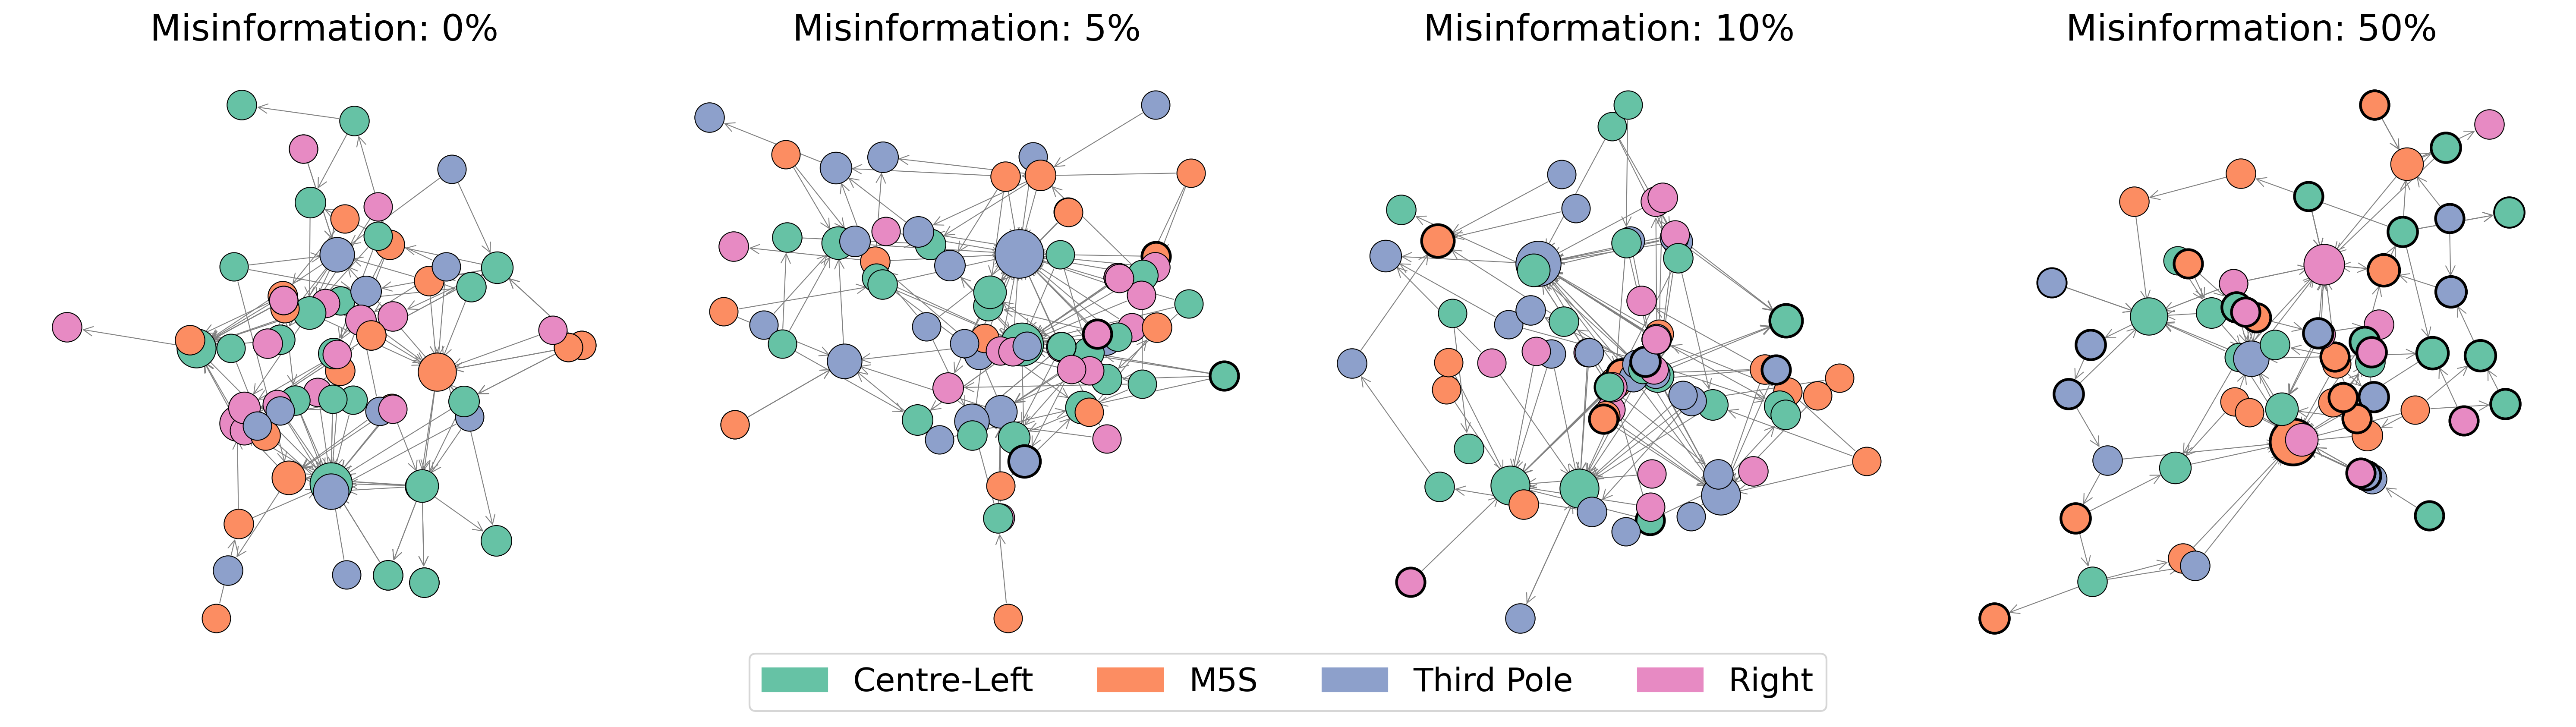
\includegraphics[width=1\linewidth]{Images/Network/graphs_DefaultRecSys.png}
    \caption{Final structure of the social network in four simulations with different levels of misinformation. 
    Nodes are agents, colored according to the supported coalition; the bold borders indicate misinformation agents. 
    The dimension of the nodes indicates the number of connections of an agent.
    The connections in the network are both in and out coalition, including misinformation agents.}
    \label{fig:network_structure}
\end{figure}


% evoluzione della rete (?)


% Opinion
\subsection{Opinion evolution}
One of the main aspects of the simulations is the evolution of opinions over time, which can be observed making a distinction for each topic and coalition.
Figure \ref{fig:opinion_evolution} shows the opinion evolution over virtual days, with a 95\% confidence interval, on each setup.
The plots on the top represent the score directly assigned by LLMs, while the ones on the bottom show the score computed with traditional opinion dynamic models.

Comparing the two score models highlights a high coherency in the trends: both scores evolves with the same behavior, and with similar mean values.
This suggests that LLMs are able to effectively replicate the opinions updates at the population level, as the observed behavior is close to that of established models in literature. Therefore, LLMs represent a valid approach in complex scenarios.

Across all topics, it's possible to observe a progressive convergence of opinions toward neutral values, indicating that agents trend to reduce their polarization over time.
It would be interesting to extend the duration of the simulations, as it would allow to determine if this trend persists or stabilizes.

Moreover, the general trend is the same even in different setups (with varying misinformation levels and different recommender systems), confirming the validity of these observations.

\begin{figure}[h]
    \centering
    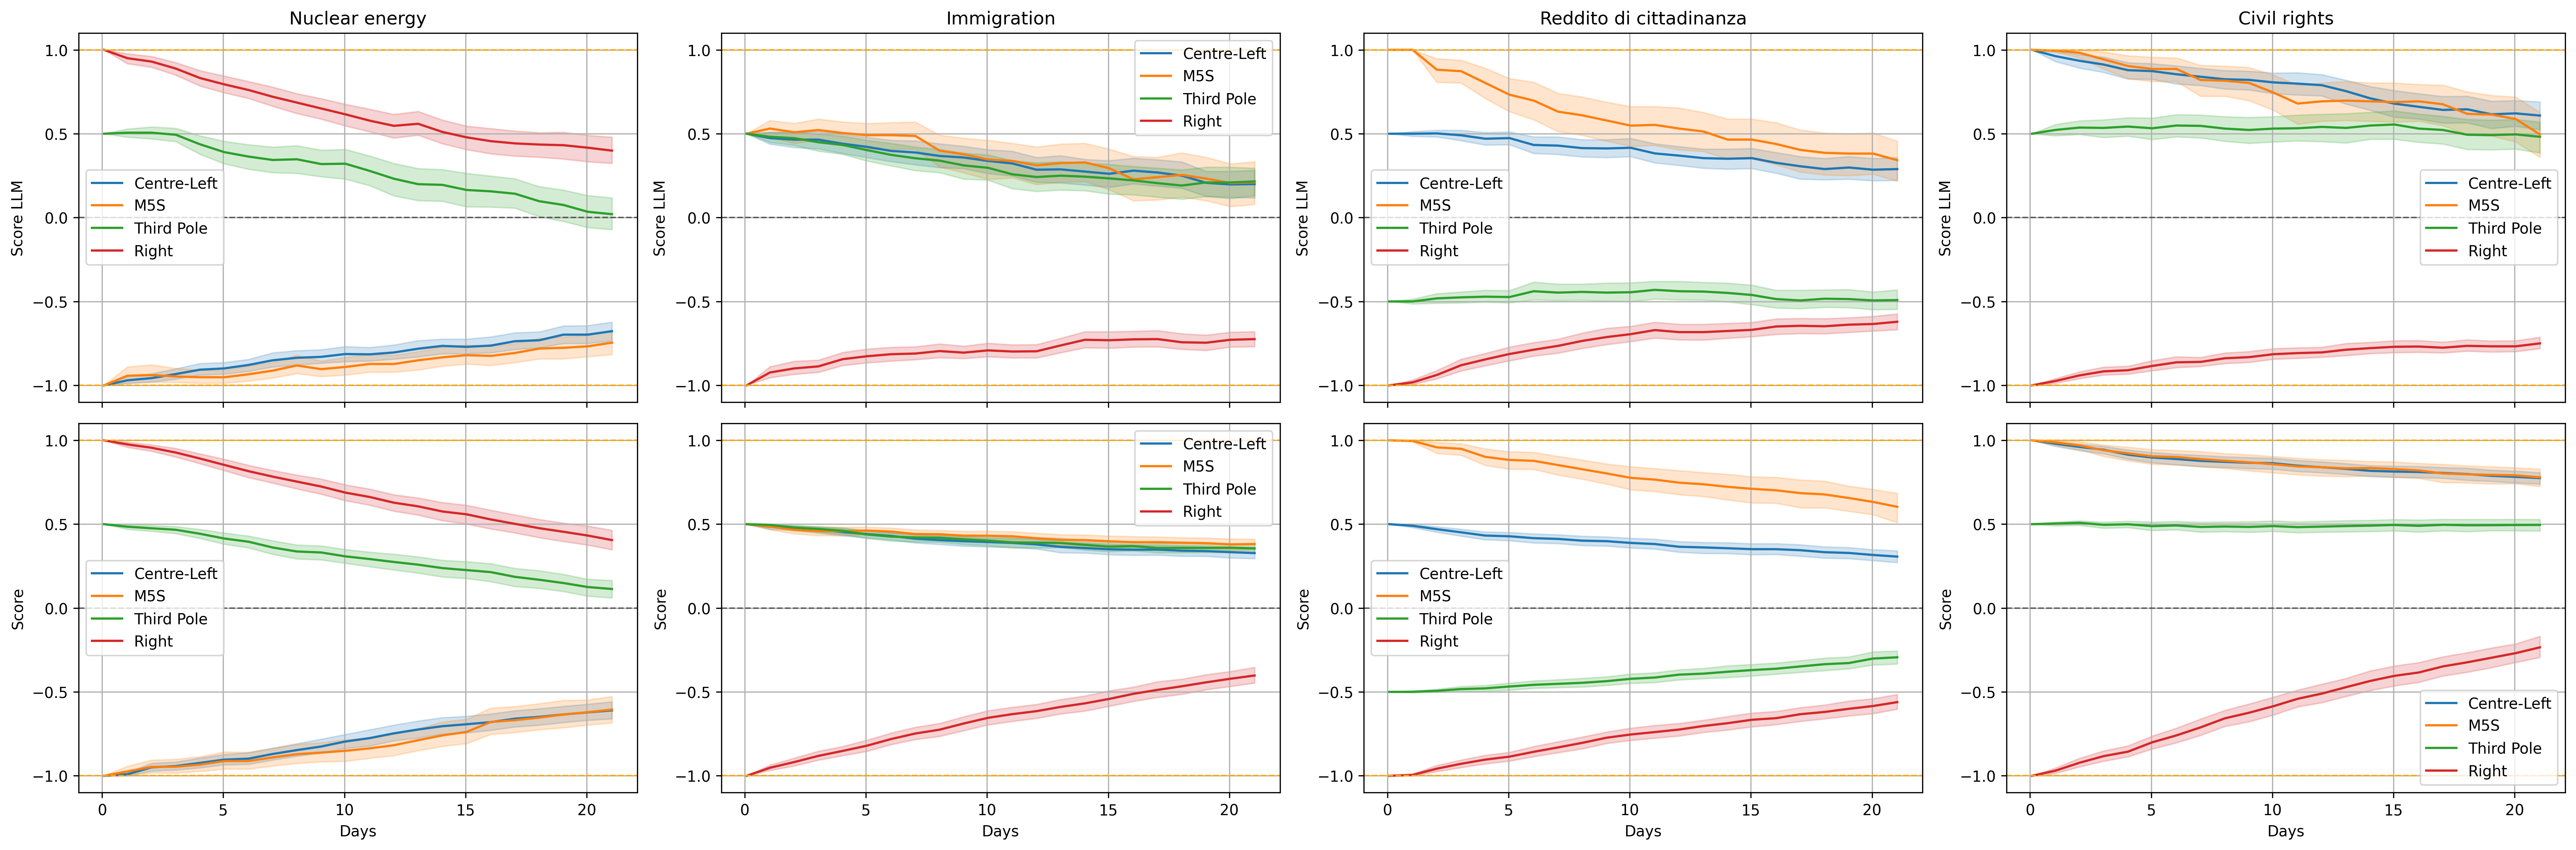
\includegraphics[width=1\linewidth]{Images/Opinions/d21a100m00d_DefaultRecSys.png}
    \caption{Evolution of opinion for each topic, comparing LLM-assigned score (\textit{score\_llm}, top row) and the one assigned by a traditional model (\textit{score}, bottom row).
    Each line represents a coalition, with a 95\% confidence interval.
    This figure is based on the runs for a single setup, but the trend is consistent with the other scenarios.}
    \label{fig:opinion_evolution}
\end{figure}


% ridge opinion shift by coalition




% Misinformation
\subsection{Misinformation}

% Toxicity analysis
\subsection{Toxicity analysis}
To analyze the toxicity of generated content, the Detoxify library \cite{hanu2020detoxify} was used. This widely adopted tool detects offensive or harmful language in text and provides a continuous toxicity score between 0 and 1.
This section explores two aspects of the toxicity in the simulations: how it varies depending on whether users interact with in-group or out-group users, and how it differs across political coalitions and content types.

\subsection{Toxicity Toward In-Group vs Out-Group}
To analyze the toxicity of comments, for each user we computed the difference between the average toxicity of replies to users from the same coalition (in-group) and those directed at users from different coalitions (out-group).
The resulting distribution is visible in Figure \ref{fig:toxicity_in_out}.
To improve readability, toxicity values were normalized according to a logarithmic scale, since original values follow an exponential distribution: $log(toxicity + 1)$.

Looking at the plot, we can see that both distributions, one for the simulated content and one for the real data, are centered around zero.
This suggests that, on average, users don't show a strong difference in behavior when replying to in-group or out-group members.

However, the distribution of the simulated data is narrower and concentrated near zero.
This means that most agents behave in a similar way, with small variations in the toxicity difference between groups.

In contrast, the real data show a wider distribution: some users are more hostile way toward other coalitions, while others show more toxic behavior toward people supporting the same coalition.
This indicates a greater variety of behaviors in real-world interactions.

It's also possible to notice that both curves have a slight shift to the right, which may suggest a slight tendency to be more toxic toward out-group members. However, this effect is minimal.

Overall, the simulations fail to reproduce the diversity of behaviors observed in real data. 
In the scenarios studies, LLMs tend to behave in a uniform way and are not able to capture the differences in hostility toward different groups.


\begin{figure}[h]
    \centering
    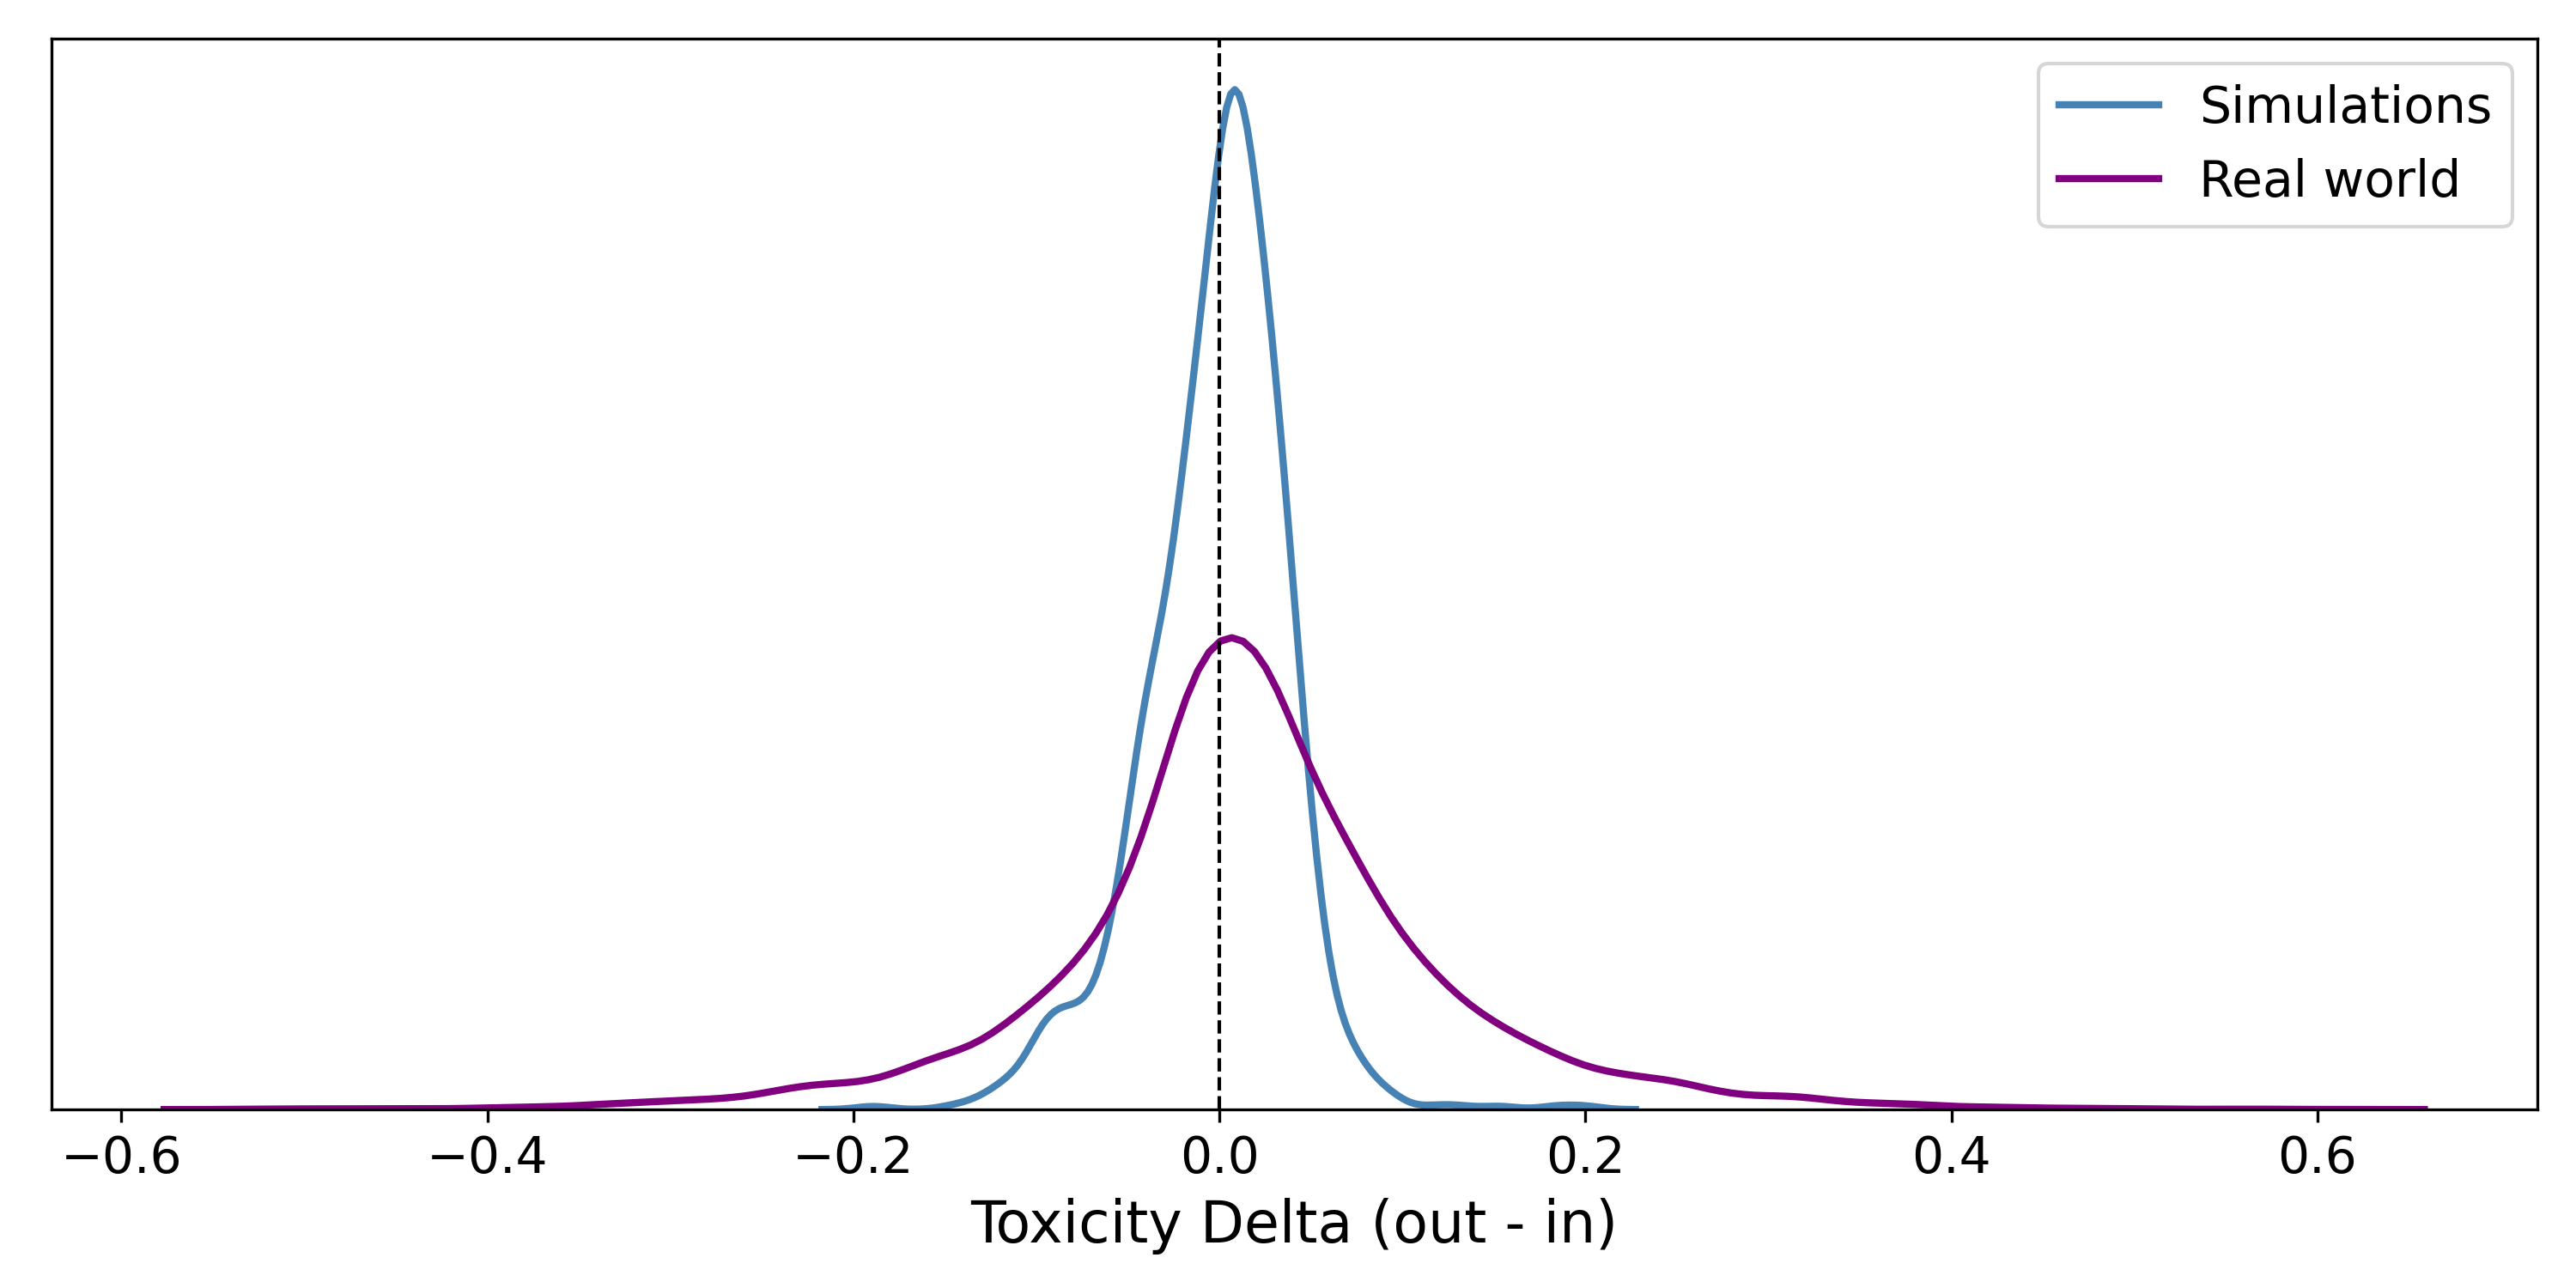
\includegraphics[width=0.6\linewidth]{Images/Toxicity/diff_in_out_combined.png}
    \caption{
    Distribution of the difference in mean toxicity toward out-group and in-group in user comments.
    The distribution of simulated content is more centered and narrow, indicating that agents behave similarly across groups.
    Real-wold data show greater variance, suggesting that some users are more hostile toward one of the two groups.
    }
    \label{fig:toxicity_in_out}
\end{figure}


\subsection{Toxicity Across Coalitions and Content Types}
The analysis of toxicity in texts generated by LLMs, divided by post and comments and categorized by political coalition, reveals some interesting dynamics in the communication style of the agents within the simulations.

In general, posts tend to be more toxic on average than comments, with an a single exception: the Right coalition.
In this case, the generated comments are more toxic than the posts, suggesting that the the Right tends to bring more conflictual contributions to the conversations.
The Right coalition also shows the greatest variance in comment toxicity.
This suggests that their replies are more heterogeneous and can include extremely toxic texts.

The M5S coalition exhibits the greatest average toxicity in posts.
In addition, the distribution shows a visible positive skew, indicating that, beyond the generally more aggressive tone, there are also occasional posts with high levels of toxicity.

In contrast, the Centre-Left and Third Pole coalitions maintain a more moderate and stable tone, across both comments and posts.

Another important insight from this analysis concerns the shape of the toxicity distribution.
In all cases, the data shows a relevant positive skew: most texts have very low toxicity, but there are long tails extending toward higher values.
This pattern becomes particularly evident when using a logarithmic scale on the y axis, which makes these cases more visible.
This suggests that, despite the generally low average toxicity, LLMs can still produce highly toxic content, even though at lower frequency.

This ability to generate even highly toxic texts, maybe facilitated by the use of an uncensored language model, is beneficial in the context of social media simulations, as it allows a more realistic modeling of online conversations.


\begin{figure}[h]
    \centering
    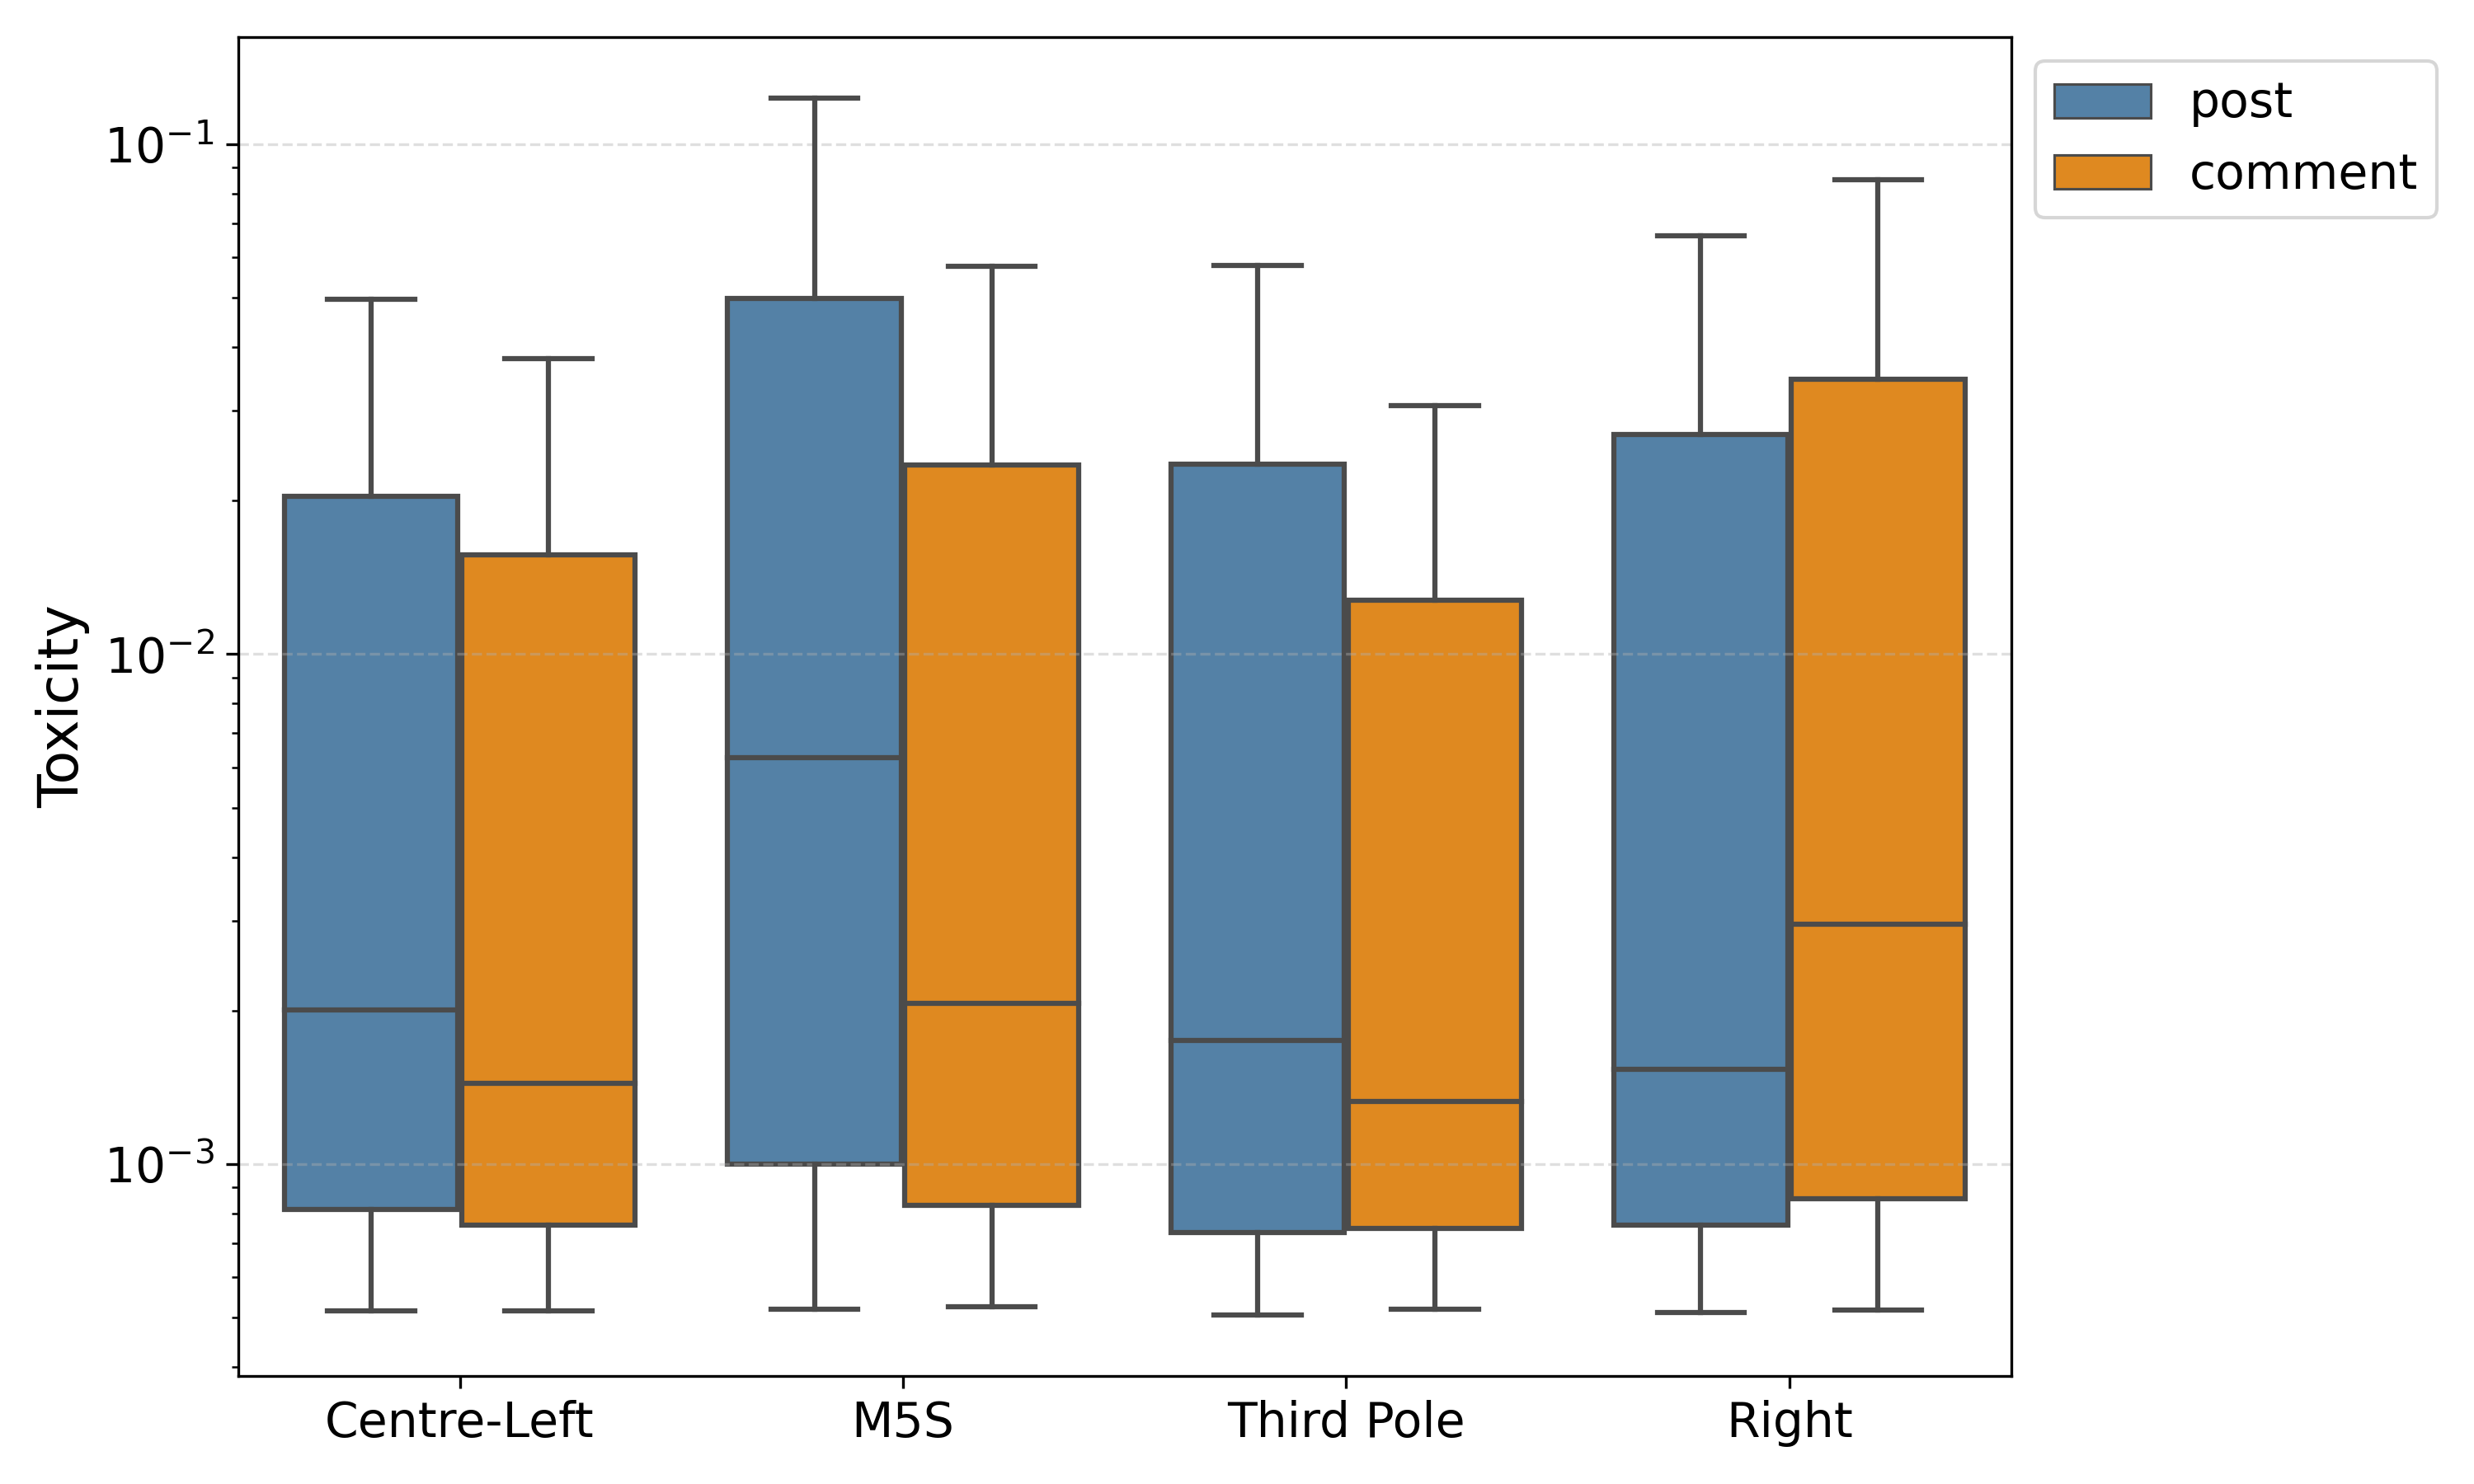
\includegraphics[width=0.6\linewidth]{Images/Toxicity/box_posts_vs_comments.png}
    \caption{
    Toxicity of LLM-generated texts, in posts and comments per political coalition.
    The y axis is in logarithmic scale to highlight the skew of the distribution.
    The Centre-Left and Third Pole coalitions have more stable and moderate tones.
    M5S is the most toxic in posts, while the Right generates comments with greater variability and toxicity.
    The long tails in all cases indicate that LLMs can generate content extremely toxic, even if rarely.
    }
    \label{fig:toxicity_in_out}
\end{figure}


% Recsys
\subsection{Content Recommendation Algorithms}
A comparison of the two content recommendation algorithms on the previously presented plots doesn't highlight any significant difference.
This happens because, at the beginning of the simulation, agents are not connected, so the network is empty.
Therefore, the used recommended system, \textit{ReverseChronoFollowersPopularity}, which should promote popular content from followers, doesn't have enough information to provide the best content.
In this initial phase, its behavior is similar to \textit{ContentRecSys}, the algorithm that suggests random content.

As a result, the different effects of the recommendation systems cannot emerge in the first few virtual days, and the dynamics produced by the two approaches are the same.
To see a real impact of the different recommender systems, simulations should run on a longer virtual time, or a network should be initialized with preexisting connections, providing a complete context of the initial user preferences.

This would allow a better evaluation of the impact of content selection on social networks.